\section*{Parsing}

In this part we take the token stream and generate an abstract syntax tree (AST).

\begin{itemize}
	\item Chomsky Hierarchy: 
		\begin{itemize}
			\item Regular - Productions have at most one nonterminal and it is at the start or end of the word
			\item Context-Free (CFG) - LHS of productions only have a single nonterminal
			\item Context-Sensitive - 
			\item Recursively Enumerable
		\end{itemize}
	
	\item A CFG consists of a set of terminals, a set of nonterminals, a start symbol and a set of productions.

	\item Derivation Orders - Productions can be applied in any order. There are two standard orders:
	\begin{itemize}
		\item Leftmost derivation: Find the left-most nonterminal and apply a production to it
		\item Rightmost derivation: Find the right-most nonterminal and apply a production there
	\end{itemize}
	All orders will lead to the same parse tree.
	
	\item A grammar is \textbf{ambiguous} if there are multiple derivation trees for the same word.
	
	\item In CFGs ambiguity can (often) be removed by encoding precedence and associativity in the grammar.
	
	\item LL \& LR Parsing
	\begin{itemize}
		\item Top-down vs. Bottom-up
		
		\item There is a problem: Want to decide which production to apply based on the look-ahead symbol $\rightarrow$ LL(1) Grammars: not all grammars can be parsed top-down with a single lookahead.
		
		\item LL(1) means \textbf{L}eft-to-right scanning, \textbf{L}eft-most derivation, \textbf{1} lookahead symbol.
		
		\item Left-factoring a grammar can make it LL(1): If there is a common prefix we can add a new non-terminal at the decision point.
		
		\item We also need to eliminate left-recursion: 
		\begin{itemize}
			\item $S \rightarrow S\; \alpha_1 \;|\; \cdots \;|\; S\; \alpha _n \;|\; \beta _1 \;|\; \cdots \;|\; \beta_m$
			
			Rewrite as
			
			$S\; \rightarrow \beta _1\; S' \;|\; \cdots \;|\; \beta _m\; S'$
			
			$S' \rightarrow \alpha_1\; S' \;|\;  \cdots \;|\; \alpha_n\; S' \;|\; \epsilon$ 
		\end{itemize}
	
		\item Predictive Parsing: Given an LL(1) grammar: For a given nonterminal, the lookahead symbol uniquely determines the production to apply - top-down parsing = predictive parsing - driven by a predictive parsing table: \textit{nonterminal x input token $\rightarrow$ production}
		
		\item Constructing the parsing table: 
		Consider a given production $A \rightarrow \gamma$
		
		(Case 1) Construct the set of all input tokens that may appear \textbf{first} in strings that can be derived from $\gamma$ - Add the production $\rightarrow \gamma$ to the entry for each such token
		
		(Case 2) If $\gamma$ can derive $\epsilon$, then we construct the set of all input tokens that may \textbf{follow} the nonterminal $A$ in the grammar - Add the production $\rightarrow \gamma$ to the entry for each such token
		
		\textbf{If there are two different productions for a given entry, the grammar is not LL(1)}
		
		\item Bottom-up Parsing, LR(k) Parser: \textbf{L}eft-to-right scanning, \textbf{R}ightmost derivation, \textbf{k} lookahead symbols
		
		LR grammars are more expressive than LL grammars. They can handle left-recursive and right-recursive grammars.
		
		Technique: "Shift-Reduce" parsers: Work bottom up and construct right-most derivation of a program in the grammar. Better error detection/recovery, but poor error reporting.
		
		Parser state: Stack of terminals and nonterminals. Unconsumed input is a string of terminals. Current derivation step is stack + input
		
		\item Shift: Move look-ahead token to the stack
		
		\item Reduce: Replace symbols $\gamma$ at the top of stack with nonterminal X s.t.  $X \rightarrow \gamma$ is a production. pop $\gamma$, push $X$. 
			
		\item Action Selection Problem:
		\begin{itemize}
			\item Given a stack $\sigma$ and a lookahead symbol $b$, should the parser \textbf{shift} $b$ onto the stack (new stack is $\sigma b$) , or \textbf{reduce} a production $X \mapsto \gamma$, assuming that $\sigma = \alpha \gamma$ (new stack if $\alpha X$)?
			\item Sometimes the parser can reduce, but should not, sometimes the stack can be reduced in different ways
			\item Main idea: Decide based on a prefix $\alpha$ of the stack plus look-ahead
		\end{itemize}
		
		\item LR(0) state: items to track progress on possible upcoming reductions.
		
		\item LR(0) item: a production with an extra separator "." in the RHS.
		
		\item The idea is that the stuff before the "." is already on the stack and the rest is what might be seen next. 
		
		\item Constructing the DFA:
		\begin{itemize}
			\item Add new production: $S' \mapsto S\$$
			
			\item Start state of the DFA = empty stack, $S' \mapsto .S\$$
			
			\item Closure:
			
			1. Adds items for all productions whose LHS nonterminal occurs in an item in the state just after the ".".
			
			2. The added items have the "." at the beginning 
		
			3. Keep iterating until a fixed point is reached.
		\end{itemize} 
		
		\item Run parser state though a DFA. DFA can be represented as a table of shape state $\times$ (terminals + nonterminals). Two types of actions: shift and go to state n, reduce using reduction $X \mapsto \gamma$
		
		\item An LR(0) machine only works if states with reduce actions have a single reduce action else we will encounter shift/reduce or reduce/reduce conflicts (use LR(1) grammar).
	\end{itemize}
\end{itemize}


\tikzset{every picture/.style={line width=0.8pt}} %set default line width to 0.75pt 

\begin{center}
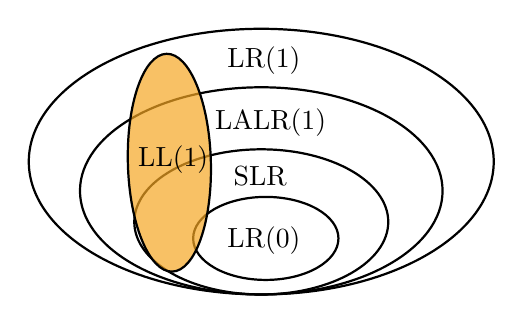
\begin{tikzpicture}[x=0.75pt,y=0.75pt,yscale=-1, xscale=1]
%uncomment if require: \path (0,719); %set diagram left start at 0, and has height of 719

%Shape: Ellipse [id:dp342446435028968] 
\draw   (505,130) .. controls (505,118.95) and (520.67,110) .. (540,110) .. controls (559.33,110) and (575,118.95) .. (575,130) .. controls (575,141.05) and (559.33,150) .. (540,150) .. controls (520.67,150) and (505,141.05) .. (505,130) -- cycle ;
%Shape: Ellipse [id:dp31528986086353894] 
\draw   (476.63,122.04) .. controls (476.63,102.73) and (504.02,87.07) .. (537.81,87.07) .. controls (571.61,87.07) and (599,102.73) .. (599,122.04) .. controls (599,141.35) and (571.61,157) .. (537.81,157) .. controls (504.02,157) and (476.63,141.35) .. (476.63,122.04) -- cycle ;
%Shape: Ellipse [id:dp8349221817367837] 
\draw   (450.47,107.09) .. controls (450.47,79.52) and (489.57,57.18) .. (537.81,57.18) .. controls (586.05,57.18) and (625.16,79.52) .. (625.16,107.09) .. controls (625.16,134.65) and (586.05,157) .. (537.81,157) .. controls (489.57,157) and (450.47,134.65) .. (450.47,107.09) -- cycle ;
%Shape: Ellipse [id:dp22985392220585588] 
\draw   (425.81,93) .. controls (425.81,57.65) and (475.96,29) .. (537.81,29) .. controls (599.67,29) and (649.81,57.65) .. (649.81,93) .. controls (649.81,128.35) and (599.67,157) .. (537.81,157) .. controls (475.96,157) and (425.81,128.35) .. (425.81,93) -- cycle ;
%Shape: Ellipse [id:dp012648097779113021] 
\draw  [fill={rgb, 255:red, 245; green, 166; blue, 35 }  ,fill opacity=0.7 ] (492.16,41.05) .. controls (503.2,40.76) and (512.77,64.01) .. (513.53,92.99) .. controls (514.3,121.97) and (505.96,145.7) .. (494.92,145.99) .. controls (483.88,146.28) and (474.31,123.02) .. (473.55,94.05) .. controls (472.78,65.07) and (481.11,41.34) .. (492.16,41.05) -- cycle ;

% Text Node
\draw (520,123) node [anchor=north west][inner sep=0.75pt]   [align=left] {LR(0)};
% Text Node
\draw (523,94) node [anchor=north west][inner sep=0.75pt]   [align=left] {SLR};
% Text Node
\draw (514,66) node [anchor=north west][inner sep=0.75pt]   [align=left] {LALR(1)};
% Text Node
\draw (520,36) node [anchor=north west][inner sep=0.75pt]   [align=left] {LR(1)};
% Text Node
\draw (477, 84) node [anchor=north west][inner sep=0.75pt]   [align=left] {LL(1)};
\end{tikzpicture}
\end{center}
